  \documentclass[a4paper, titlepage]{report}
\usepackage[utf8]{inputenc}
\usepackage[T1]{fontenc}
\usepackage[french]{babel}

\usepackage{graphicx} 


\usepackage{lmodern} % Pour changer le pack de police
\usepackage[vlined, longend]{algorithm2e}
\usepackage{multicol}
\usepackage[a4paper, top=2cm, bottom=2cm, left=2cm, right=2cm]{geometry}


\usepackage{wrapfig}
 


\setlength{\algomargin}{0em}
\SetKwRepeat{Repeat}{Do}{While}
\SetKwIF{If}{ElseIf}{Else}{If}{then}{Else if}{Else}{EndIf}
\SetKwFor{For}{For}{do}{Done}
\SetKwFor{While}{While}{do}{Done}

\providecommand{\SetAlgoLined}{\SetLine}
\providecommand{\DontPrintSemicolon}{\dontprintsemicolon}

\SetKwBlock{Begin}{Begin}{End}

\SetKw{KwFrom}{from }
\SetKw{KwBy}{by }
\DontPrintSemicolon	% do not print the ';' symbol
\newcommand{\TRUE}{\textit{TRUE} }
\newcommand{\FALSE}{\textit{FALSE} }
\newcommand{\AND}{\textit{AND} }
\newcommand{\OR}{\textit{OR} }
\newcommand{\NULL}{\textit{NULL} }

\newcommand{\NewWhile}{\SetKwBlock{While}{while}{}}
\newcommand{\NormalWhile}{\SetKwBlock{While}{while}{Done}}

\setcounter{secnumdepth}{5}
\setcounter{tocdepth}{5}

\newenvironment{lexicon}{\noindent \hspace{1.2em} {\bf \underline{Lexicon}} \\~\\}{ ~\\ }
\newenvironment{algo}{\noindent \hspace{1.2em} {\bf \underline{Algorithm}} \\~\\ \begin{algorithm}[H] \SetAlgoLined }{\end{algorithm}  ~\\}

\usepackage{listings}
\lstset{ 
language=java
}

\title{LO43 
     Flotte de véhicules autonomes}
\author{Buri Theo florian Lacour} 
\date{Hiver 2013}

\makeatletter
\def\clap#1{\hbox to 0pt{\hss #1\hss}}%
\def\ligne#1{%
\hbox to \hsize{%
\vbox{\centering #1}}}%
\def\haut#1#2#3{%
\hbox to \hsize{%
\rlap{\vtop{\raggedright #1}}%
\hss
\clap{\vtop{\centering #2}}%
\hss
\llap{\vtop{\raggedleft #3}}}}%
\def\bas#1#2#3{%
\hbox to \hsize{%
\rlap{\vbox{\raggedright #1}}%
\hss
\clap{\vbox{\centering #2}}%
\hss
\llap{\vbox{\raggedleft #3}}}}%
\def\maketitle{%
\thispagestyle{empty}\vbox to \vsize{%
\haut{}{\@blurb}{}
\vfill
\vspace{1cm}
\begin{flushleft}
\usefont{OT1}{ptm}{m}{n}
\huge \@title
\end{flushleft}
\par
\hrule height 4pt
\par
\begin{flushright}
\usefont{OT1}{phv}{m}{n}
\Large \@author
\par
\end{flushright}
\vspace{1cm}
\vfill
\vfill
\bas{}{\@location, \@date}{}
}%
\cleardoublepage
}
\def\date#1{\def\@date{#1}}
\def\author#1{\def\@author{#1}}
\def\title#1{\def\@title{#1}}
\def\location#1{\def\@location{#1}}
\def\blurb#1{\def\@blurb{#1}}
\date{Décembre 2014}
\author{}
\title{}
\makeatother
\title{LO43 Flotte de véhicule autonomes}
\author{Buri Theo Florian Lacour}
\location{Belfort}
\blurb{%
Université de technologie de Belfort-Montbéliard
}% 

\usepackage{array}


\begin{document}


\maketitle
\tableofcontents
\newpage
\chapter*{Introduction}
\addcontentsline{toc}{chapter}{Introduction}
\hspace{0.5cm}Dans le cadre de  l'UV LO43 " Bases fondamentales de la programmation orientée objet", il nous a été demandé de réaliser un projet de groupe, afin de mettre en pratique les connaissances acquises lors des cours et TDs du semestre.
\\
Trois sujet nous on été présentés. Nous avons fait le choix de traiter le sujet de la "Flotte de véhicules autonomes", et ceci pour plusieurs raisons :
\begin{itemize}
  \item (A TROUVER)
  \item N'étant que deux, sur un maximum de quatre étudiants par groupe autorisés, les autres sujets ne nous ont pas parus réalisables en temps et en heures et sans bugs majeurs...
  \item (A TROUVER)
\end{itemize}
\end
Dans un premier temps, nous feront une présentation du sujet choisi, puis nous présenterons les diagramme UML, pour enfin vous presenter notre implémentation en JAVA.
\part{ Description du sujet}
\section{Objectif}
 L'application a réaliser est la modélisation d'une flotte de véhicules évoluant dans une infrastructure de circulation partagé. Pour cela nous devont modéliser la parti modèle notre programme a l'aide d'UML qui est un  langage de modélisation graphique à base de pictogrammes. Puis nous implémenteront cette modélisation en JAVA.
 \\
 
\section{Reformulation du sujet}
Le plateau donné par le sujet et le suivant :
 \\
 \\

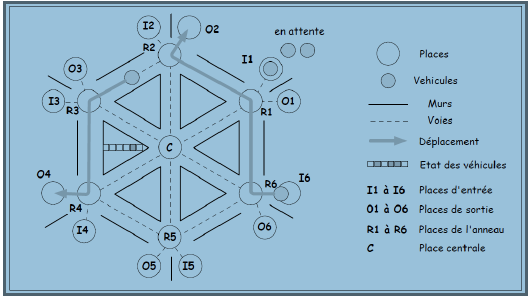
\includegraphics[]{Images/Plateau}
\\
\\
De plus ce sont les voitures qui doivent décide du moment ou elles partent, pour cella elle doivent envoyer une requête au contrôleur pour savoir si leur chemin est déjà réserver. Afin d'éviter toute erreur lors de la réservation nous avons défini un ordre tel qui suit: 
			I1<I2<I3<I4<I5<I6<R1<R2<R3<R4<R5<R6<O1<O2<O3<O4<O5<O6< C
De plus les voiture ne peuvent prendre la place central qu'a la seul condition quel doivent aller a la place en face de la leurs.
Cette requête est implémenter sous forme de bitmap.

Par exemple pour une voiture qui désire aller de la place I1 a O2 la request map seras la suivante.




\begin{tabular}{|l|l|l|l|l|l|l|l|l|l|l|l|l|l|l|l|l|l|l|l|}

\hline
  I1 & I2 & I3 & I4 & I5 & I6 & R1 & R2 & R3 & R4 & R5 & R6 & O1 & O2 & O3 & O4 & O5 & O6 & C \\
  \hline
   T & F & F & F & F & F & T & T & F & F & F & F & F & T & F & F & F & F & F\\
 \hline

\end{tabular}


\end{document}